\documentclass[11pt]{article}
\usepackage{graphicx}
\usepackage[bookmarks=true]{hyperref}
\usepackage{bookmark}
\usepackage{hyperref}
\usepackage{float}
\usepackage{wrapfig}

\usepackage{array}
\newcolumntype{L}[1]{>{\raggedright\let\newline\\\arraybackslash\hspace{0pt}}m{#1}}
\newcolumntype{C}[1]{>{\centering\let\newline\\\arraybackslash\hspace{0pt}}m{#1}}
\newcolumntype{R}[1]{>{\raggedleft\let\newline\\\arraybackslash\hspace{0pt}}m{#1}}

\begin{document}

\begin{titlepage}
\begin{flushright}


\includegraphics[width=380px]{./images/University_of_Pretoria_Logo.png}
\newline
\newline

\textbf {\LARGE Software Requirements Specification} \newline

\textbf {\Large Linphone for Andriod Group Chat (Waterfall)}\newline

\textbf {\large Version: 2.0}\newline

\centering \textbf {\large Authors:}

\begin{table}[H]
\large
\centering
\begin{tabular}{rl}
	Izak Blom & 13126777 \\
	David Breetzke & 12056503 \\
	Paul Engelke & 13093500 \\
	Prenolan Govender & 13102380 \\
	Jessica Lessev & 13049136 \\
\end{tabular}
\end{table}

Date: 26 May 2015

\end{flushright}
\end{titlepage}

\setcounter{tocdepth}{3}
\tableofcontents

\newpage
\section{Revision History}
\begin{table}[h]
\begin{tabular}{llll}
\textbf{Date}          & \textbf{Description}  & \textbf{Author}       & \textbf{Comments}   \\ \hline
\multicolumn{1}{|R{2.5cm}|}{26/05/2015} & \multicolumn{1}{L{5.5cm}|}{Document Creation} & \multicolumn{1}{l|}{Team Eclectic} & \multicolumn{1}{L{4cm}|}{Version 1} \\ \hline
\multicolumn{1}{|l|}{} & \multicolumn{1}{l|}{} & \multicolumn{1}{l|}{} & \multicolumn{1}{l|}{} \\ \hline
\multicolumn{1}{|l|}{} & \multicolumn{1}{l|}{} & \multicolumn{1}{l|}{} & \multicolumn{1}{l|}{} \\ \hline
\multicolumn{1}{|l|}{} & \multicolumn{1}{l|}{} & \multicolumn{1}{l|}{} & \multicolumn{1}{l|}{} \\ \hline
\multicolumn{1}{|l|}{} & \multicolumn{1}{l|}{} & \multicolumn{1}{l|}{} & \multicolumn{1}{l|}{} \\ \hline
\multicolumn{1}{|l|}{} & \multicolumn{1}{l|}{} & \multicolumn{1}{l|}{} & \multicolumn{1}{l|}{} \\ \hline
\multicolumn{1}{|l|}{} & \multicolumn{1}{l|}{} & \multicolumn{1}{l|}{} & \multicolumn{1}{l|}{} \\ \hline
\multicolumn{1}{|l|}{} & \multicolumn{1}{l|}{} & \multicolumn{1}{l|}{} & \multicolumn{1}{l|}{} \\ \hline
\multicolumn{1}{|l|}{} & \multicolumn{1}{l|}{} & \multicolumn{1}{l|}{} & \multicolumn{1}{l|}{} \\ \hline
\multicolumn{1}{|l|}{} & \multicolumn{1}{l|}{} & \multicolumn{1}{l|}{} & \multicolumn{1}{l|}{} \\ \hline
\end{tabular}
\end{table}

\section{Document Approval}
\begin{table}[h]
\begin{tabular}{llll}
\textbf{Signature}     & \textbf{Printed Name} & \textbf{Title}        & \textbf{Comments}     \\ \hline
\multicolumn{1}{|l|}{} & \multicolumn{1}{L{4.5cm}|}{} & \multicolumn{1}{L{4cm}|}{} & \multicolumn{1}{L{4cm}|}{} \\ \hline
\multicolumn{1}{|l|}{} & \multicolumn{1}{l|}{} & \multicolumn{1}{l|}{} & \multicolumn{1}{l|}{} \\ \hline
\multicolumn{1}{|l|}{} & \multicolumn{1}{l|}{} & \multicolumn{1}{l|}{} & \multicolumn{1}{l|}{} \\ \hline
\multicolumn{1}{|l|}{} & \multicolumn{1}{l|}{} & \multicolumn{1}{l|}{} & \multicolumn{1}{l|}{} \\ \hline
\multicolumn{1}{|l|}{} & \multicolumn{1}{l|}{} & \multicolumn{1}{l|}{} & \multicolumn{1}{l|}{} \\ \hline
\multicolumn{1}{|l|}{} & \multicolumn{1}{l|}{} & \multicolumn{1}{l|}{} & \multicolumn{1}{l|}{} \\ \hline
\multicolumn{1}{|l|}{} & \multicolumn{1}{l|}{} & \multicolumn{1}{l|}{} & \multicolumn{1}{l|}{} \\ \hline
\multicolumn{1}{|l|}{} & \multicolumn{1}{l|}{} & \multicolumn{1}{l|}{} & \multicolumn{1}{l|}{} \\ \hline
\multicolumn{1}{|l|}{} & \multicolumn{1}{l|}{} & \multicolumn{1}{l|}{} & \multicolumn{1}{l|}{} \\ \hline
\multicolumn{1}{|l|}{} & \multicolumn{1}{l|}{} & \multicolumn{1}{l|}{} & \multicolumn{1}{l|}{} \\ \hline
\end{tabular}
\end{table}

\newpage
\section{Introduction}

\subsection{Purpose}
This document provides a detailed discussion of the Linphone Group Chat Extension system requirements and behaviour, in preparation for design and implementation. These requirements include use cases, functional and non-functional requirements as well as a description of the adjustments to be made to the existing user interfaces.
\subsection{Scope}
%The scope of this documentation is to cover all use cases and functional requirements that are necessary to provide group chat functionality to the Linphone service. \newline
%The scope of ManageGroups is restricted to creating, deleting and removing groups. These are further split up into lower-level use cases that are needed in order to achieve the desired functionality.
The scope of the Linphone Group Chat Extension is as follows:
\begin{itemize}
\item providing group chat capabilities such as:
\subitem  - creation and deletion of groups,
\subitem  - adding and removing members,
\subitem  - broadcasting all messages to all members,
\item sending messages using AES256 encryption for secure messaging,
\item sending messages without encryption where it is not needed,
\item sending voice recordings over IM,
\item making changes to the messaging user interface such as:
\subitem  - improving the spacing between words,
\subitem  - increasing the font sizes,
\subitem  - improving message indentation for sender clarity,
\subitem  - adding indication of another user typing a message,
\subitem  - improving user profile picture displays.
\end{itemize}
\begin{figure}[H]
\centering
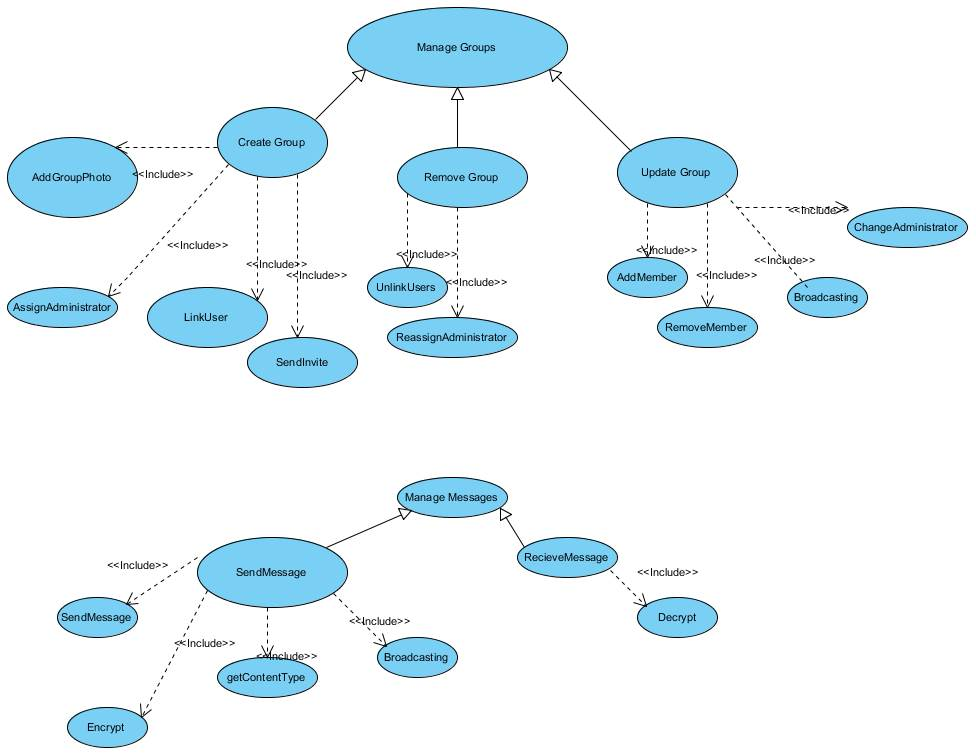
\includegraphics[width=380px]{./images/scope.jpg}
\caption[Project Scope]{This UML diagram provides the scope for the Linphone Group Chat Extension}
\label{figure-scope-master}
\end{figure}
\subsection{Definitions, Acronyms \& Abbreviations}
\subsubsection{Internal Documentation}
\paragraph{FR:} Functional Requirement
\paragraph{UC:} Use Case
\subsubsection{External Documentation}
\paragraph{AES256:} AES stands for Advanced Encryption Standard and is a specification for encryption of electronic data. AES256 is a specific encryption algorithm that uses block sizes of 256 bits.
%\subsection{References}
\subsection{Overview}

\section{Specific Requirements}
%\subsection{External Interface Requirements}
\subsubsection{User Interfaces}
 % user interface changes

%\subsubsection{Hardware Interfaces}
%\subsubsection{Software Interfaces}
%\subsubsection{Communication Interfaces}

\subsection{Use Cases}
\subsubsection{Create Group Chat} \label{UC-create-group}
\paragraph{Priority:}Critical
\paragraph{Summary:}
\paragraph{Rationale:}
\paragraph{Users:}
\paragraph{Preconditions:}
\paragraph{{Postconditions:}}
%\includegraphics[]{name} -- for use case diagram
\subsubsection{Delete Group Chat} \label{UC-delete-group}
\paragraph{Priority:}Critical
\paragraph{Summary:}
\paragraph{Rationale:}
\paragraph{Users:}
\paragraph{Preconditions:}
\paragraph{{Postconditions:}}
%\includegraphics[]{name} -- for use case diagram
\subsubsection{Update Group Chat Profile} \label{UC-update-group}
\paragraph{Priority:} Important
\paragraph{Summary:}
The group name, subject, and profile picture can be changed.
\paragraph{Rationale:}
The nature of groups can change when members are added or removed, resulting in name and subject changes. Users tend to update profile pictures often in order to keep groups from growing stale or to have the picture relate to the group name or subject. Allowing users to update features of the group will allow groups to be easier to manage and usable in terms of aesthetics.
\paragraph{Users:}
Any member of the group.
\paragraph{Preconditions:}
A group exists and has members.
\paragraph{{Postconditions:}}
The current name, subject, or profile picture has been changed.
%\includegraphics[]{name} -- for use case diagram
\subsubsection{Add Member} \label{UC-add-member}
\paragraph{Priority:} Critical
\paragraph{Summary:}
A user is added to the list of users currently in the group.
\paragraph{Rationale:}
The group does not have a static amount of users, this is inefficient. If the creator of the group has forgotten to add a user to the group after initial creation, the creator should still be able to add the user later. Should a user relevant to the group appear after creation of the group, the user should still be able to join the group. In addition, should a user leave, the user should be able to come back to the group.
\paragraph{Users:}
Creator or the current administrator of the group.
\paragraph{Preconditions:}
Group exists with an administrator in it.
\paragraph{{Postconditions:}}
The user is added to the list of current users in the group and receives messages, etc.
%\includegraphics[]{name} -- for use case diagram
\subsubsection{Remove Member} \label{UC-remove-member}
\paragraph{Priority:} Critical
\paragraph{Summary:}
A user is removed from the list of users currently in the group.
\paragraph{Rationale:}
Should a user be added to the group accidentally, it should be possible to remove said user. Users should additionally be able to remove themselves from the group should they no longer require it. Being able to remove users and users being able to remove themselves aides in the management of the group.
\paragraph{Users:}
All users. (Administration can remove other users, all users can remove themselves.)
\paragraph{Preconditions:}
A group exists with more than one member.
\paragraph{{Postconditions:}}
The user is no longer a part of the group which entails the user not receiving messages from the group, etc.
%\includegraphics[]{name} -- for use case diagram
\subsubsection{Change Administrator} \label{UC-change-admin}
\paragraph{Priority:} Important
\paragraph{Summary:}
Removes administrator privileges from the current administrator and reassigns to another user within the group.
\paragraph{Rationale:}
If a user prefers not to be administrator anymore or the current administrator would like to leave the group, assigning a new user within the group with administrator privileges makes management of the group easier.
\paragraph{Users:}
Administrator of the group.
\paragraph{Preconditions:}
Group exists with an administrator and at least one other user.
\paragraph{{Postconditions:}}
The user selected receives administrator privileges while the current administrator is stripped of the privileges.
%\includegraphics[]{name} -- for use case diagram
\subsubsection{Send Message} \label{UC-send-message}
\paragraph{Priority:} Critical
\paragraph{Summary:} The message object shall be broadcast to all participants of the group chat.
\paragraph{Rationale:} The purpose of a group chat is to provide a central point of communication for a group of people. A user should thus be able to convey a message to all other participant users in one single action.
\paragraph{Users:} Any registered member of the group chat.
\paragraph{Preconditions:} 
\begin{itemize}
\item The user is a member of the group chat.
\item The interface that has focus, is the group chat interface.
\end{itemize}
\paragraph{{Postconditions:}}
\begin{itemize}
\item The user's message has been sent to all other participants.
\end{itemize}
%\includegraphics[]{name} -- for use case diagram
\subsubsection{Send Voice Recording} \label{UC-send-voice}
\paragraph{Priority:} Important
\paragraph{Summary:} A user will be able to record voice messages and send them via IM.
\paragraph{Rationale:} A user may be pressed for time, unable type a message, or the recipient may be unable to read the message, due to some external factor and thus require a means other than text messaging to convey a message. The ability to record one's voice and send the recording as a message may cater for the described scenarios and more.
\paragraph{Users:} Any user of the Linphone application.
\paragraph{Preconditions:} The user's device must support voice recording --- the device requires a microphone to support this.
\paragraph{{Postconditions:}} A message has been sent to the recipient containing the voice recording.
%\includegraphics[]{name} -- for use case diagram

\subsection{Functional Requirements}
\subsubsection{Create Group Chat} \label{FR-create-group}
The ManageGroups module provides services to create, update and remove or leave groups.\newline
\textbf{Description:} The user activates the createGroup functionality by selecting an option to create a new group chat. The system will provide the user with a screen where details about the group such as group photo, group name and group members need to be specified. If all pre-conditions are met then the group is created. It allows for all added members to exchange messages and communicate in a common space.\newline
\newline
\begin{itemize}
\item ManageGroups.CreateGroup – Priority: Critical.
\item	This use case allows users to create a group where more than 1 contact can communicate simultaneously together.
\item	This creates a space where messages can be exchanged between users that are members of the groups.
\end{itemize}
\textbf{Services Contract:} \newline
	\newline
\begin{itemize}
\item The CreateGroupRequest identifies the user that is creating the group and automatically assigns this user to be the administrator.
\item It allows the user to select contacts that the user wishes to add to the group.
\item The group members are then notified by receiving an invitation to join and are linked to the group.
\item The service has three pre-conditions and three post-conditions
\end{itemize}
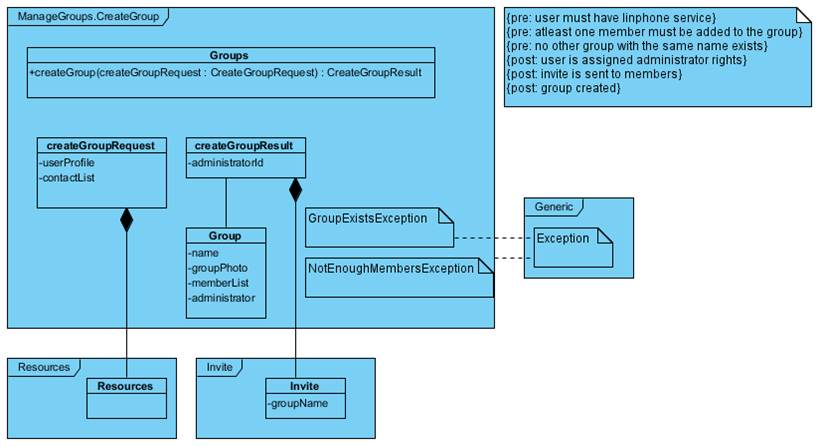
\includegraphics[width=380px]{./images/serviceContract-create.jpg} \newline
\textbf{Pre-conditions} \newline
For each of the pre-conditions below an exception is introduced which is raised by the service to notify the caller that the service is not being provided as the pre-condition associated with that exception has not been met.\newline
The group will not be created if one of the following scenarios occurs:\newline
\newline
\begin{itemize}
\item	User must have Linphone Service\newline
\item	No other group with the same name may exist \newline
\item	The user may not create the group unless there is at least one member/contact added.\newline
\end{itemize}
\textbf{Post-Conditions}\newline
The post-conditions specify the conditions which must hold true when the service has been provided.\newline
\newline
\begin{itemize}
\item	User is automatically assigned administrator rights
\item	An invite is sent to users to ask them if they want to be part of the group
\item	The group is created with the respective profiles and members
\end{itemize}
\textbf{Functional Requirements}\newline
 The functional requirements specify what the system should do and how the system should behave. Each use case has functional requirements and these specify the functions required by the use cases in order to use the service specified in the services contract. Each functional requirement is either checking for a post-condition or a precondition or both.\newline
 \newline
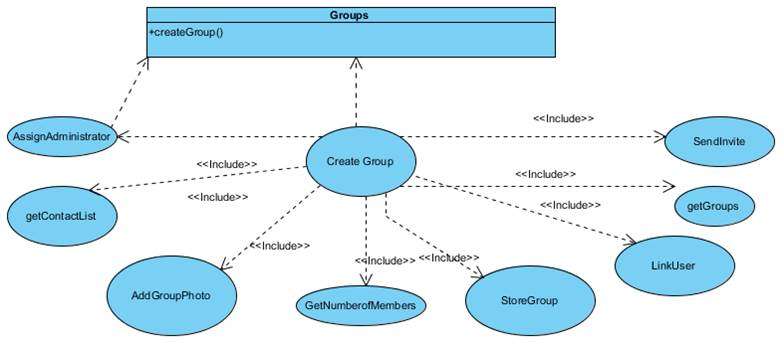
\includegraphics[width=380px]{./images/FR-create.jpg}
 \newline
\textbf{Process Specification} \newline
 \newline
 \includegraphics[width=380px]{./images/process-create.jpg}
  \newline
 First the user creating the group fills in the relative details such as the group name and adds members to the group. Each of these members needs to have the Linphone service to be added to the group. If the contacts do not have Linphone, an error is thrown. Next the user tries to create the group. If less than 1 member is added then an error is thrown and the group is not created. If more than one member was added then the system continues to check whether there are any other groups with the same name. If so, then an exception is thrown, otherwise the user is assigned as group administrator, an invite is sent to the members and the group is created.\newline
 \newline
 \textbf{Included Use cases} \newline
 Use cases that are included are necessary to provide the lower level functionality needed in order to achieve the higher level functionality. These all deal with the resources and retrieving from storage. They  are:\newline
 \newline
 \textbf{addGroupPhoto  – Priority: Important} \newline
 \begin{itemize}
 \item	This use case allows a member of the group and the administrator, on group creation, to add a group photo. On group creation, if the creator does not specify a group photo, a default one is assigned.\newline
 \end{itemize}
 \textbf{getContactList – Priority: Important} \newline
 \begin{itemize}
 \item	This use case gets the user trying to create the group’s contact list and checks whether each contact added to the group has Linphone or not. If not an exception is thrown otherwise the system proceeds further.\newline
 \end{itemize}
 \textbf{getGroups  – Priority: Critical} \newline
 \begin{itemize}
\item	This use case gets all the group names that the creator has in their chats list and checks that another group with the same name as the new group exists. If another group exists then an exception is thrown otherwise the system proceeds further. \newline
\end{itemize}
 \textbf{sendInvite – Priority: Critical} \newline
 This use case is triggered when a group is created and when new members are added to the group.  \newline 
\textbf{Services Contract:}
 \begin{itemize}
 \item	This use case contains the invite itself as well as information regarding where to send it etc.\newline
 \end{itemize}
\textbf{Pre-conditions} \newline
 For each of the pre-conditions below an exception is introduced which is raised by the service to notify the caller that the service is not being provided as the pre-condition associated with that exception has not been met.\newline
 The invite will not be sent if one of the following scenarios occurs:
 \begin{itemize}
 \item	The receiver of the invite is not a contact added by the administrator of the group.
 \end{itemize}
\textbf{Post-conditions} \newline
 The post-conditions specify the conditions which must hold true when the service has been provided.
 \begin{itemize}
\item	The invite must be sent to the correct user.
\end{itemize}
 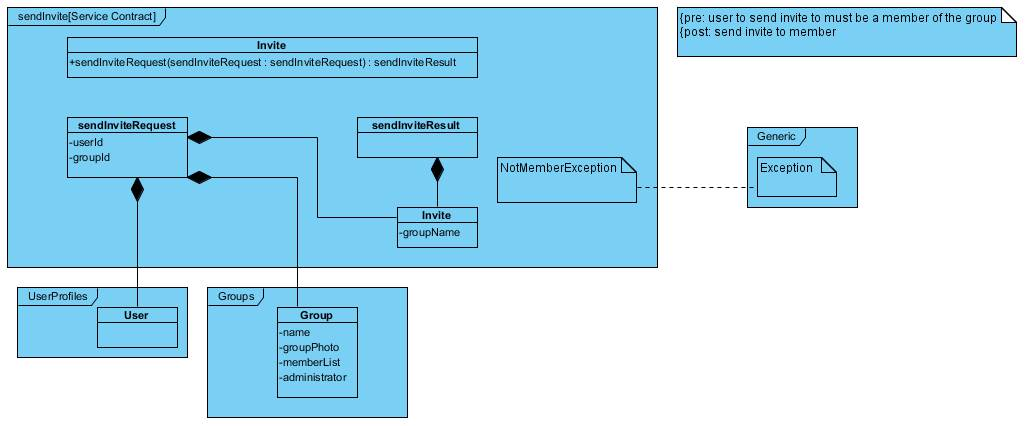
\includegraphics[width=380px]{./images/serviceContract-sendInvite.jpg} \newline
\textbf{Functional Requirements}\newline
 The functional requirements specify what the system should do and how the system should behave. Each use case has functional requirements and these specify the functions required by the use cases in order to use the service specified in the services contract. Each functional requirement is either checking for a post-condition or a precondition or both.\newline
 \newline
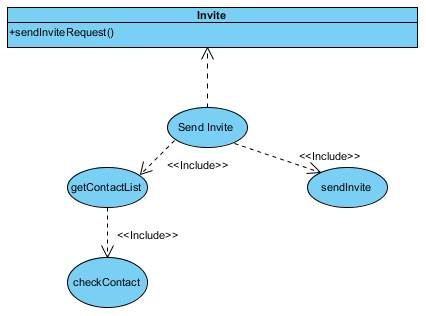
\includegraphics[width=200px]{./images/FR-sendInvite.jpg}
 \newline
\textbf{Process Specification} \newline
 \newline
 \includegraphics[width=200px]{./images/process-sendInvite.jpg}
  \newline
 
\subsubsection{Delete Group Chat} \label{FR-delete-group}
\paragraph{Summary:}
\paragraph{Rationale:}
\paragraph{Requirements:}
\paragraph{References:} UC \ref{UC-delete-group}
\subsubsection{Update Group Profile Picture} \label{FR-update-group-picture}
\paragraph{Summary:}
Updating should allow a user to remove the profile picture from the group or choose an image from local storage to replace the current profile picture.
\paragraph{Rationale:}
A user will often change the profile picture of the group, allowing the user to choose an image from local storage will afford the user more options.
\paragraph{Requirements:}
When the user chooses to change the profile picture, the user must be afforded the option to remove the profile picture (replacing it with a default system image) or allow the user to choose a new picture by invoking the file manager in order to choose a picture from local storage. The updated profile picture should be visible to all users within the group after the change has taken place.
\paragraph{References:} UC \ref{UC-update-group}
\subsubsection{Add Member} \label{FR-add-member}
\paragraph{Summary:}
Once the user has been added to the group, the user must be able to receive messages from the group and other members.
\paragraph{Rationale:}
Users will be added at different times to other users therefore it must be guaranteed that each user receives the same messages as other group members.
\paragraph{Requirements:}
Once the administrator opts to add a user, the list of contacts the user currently has must appear and the user can choose another user to add to the group. When the user is selected, that user must be added to the group list and receive all messages sent in the group from that point.
\paragraph{References:} UC \ref{UC-add-member}
\subsubsection{Remove Member} \label{FR-remove-member}
\paragraph{Summary:}
Once the user has been removed from the group, the user must not receive any messages from the group.
\paragraph{Rationale:}
Users will be removed at different times to other users therefore it must be guaranteed that the user who is removed does not receive any messages from the group to ensure that the user is not a part of the group.
\paragraph{Requirements:}
Once the administrator opts to remove a user from the list of users currently in the group, the user selected must be removed from the group and should no longer receive any messages from the group.
\paragraph{References:} UC \ref{UC-remove-member}
\subsubsection{Encryption for Send Message} \label{FR-send-message-encrypted}
\paragraph{Summary:} The send message feature shall provide for encryption.
\paragraph{Rationale:} If the group administrator decides that messages should be encrypted for secure communication amongst members, the ability to do so shall be provided.
\paragraph{Requirements:} When encryption is enabled, the send message feature shall use the AES265 encryption algorithm to encrypt the message before broadcasting it to the group members. If encryption is not enabled, the message will be broadcast in it's original state.
\paragraph{References:} UC \ref{UC-send-message}
\subsubsection{Voice Recording Support} \label{FR-voice-record-support}
\paragraph{Summary:} The voice recording feature shall check that the device has a microphone.
\paragraph{Rationale:} The voice recording feature can only operate if it can receive audio input from the device's microphone. Without such a check, trying to access the feature can lead to the possibility of a system crash.
\paragraph{Requirements:} When the voice recording feature is invoked, the procedure will check that the device can record audio. If it can, it will proceed with normal execution: using the device microphone to record the audio and once done, wrap the audio file in a message object and send it; else it will abort the process and alert the user that the feature is not available.
\paragraph{References:} UC \ref{UC-send-voice}

\subsection{Non-Functional Requirements}
\subsubsection{Scalability Constraints for Add User} \label{NF-performance-add-member}
\paragraph{Summary:} Adding a new user may not negatively impact the performance of management of, and communication within, the group.
\paragraph{Rationale:} If there are too many members in a group, it can become hard for the group administrator to keep track of members and there may be noticeable delays in message broadcasting with some users receiving messages much later than others. This can impact the service quality negatively cause people to stop using the service.
\paragraph{Requirements:} The number of users per group shall be limited to a reasonable size to prevent poor performance. This number should be between 50 and 100 users, although this number is subject to change as development and testing progress.
\paragraph{References:} UC \ref{UC-add-member}

\subsubsection{Performance Constraints for Send Message}

%\section{Requirements Traceability Matrix}

\newpage
\section{Appendix A} \label{appendix-a}
\listoffigures

\end{document}